%XXX Since design will focus on each component, this section can mirror the previous chapter, but instead of high level overview, describe how you implemented the description from the design chapter, programming language, libraries etc.

\chapter{Implementation of \project}\label{ch:implementation}\glsresetall
This chapter describes the implementation of \project. First we will go through the programming language and modules we use. Then we will detail the implementation of each component.

We implement \project in the programming language \href{https://www.python.org/}{Python}, which is a powerful high-level scripting language that is excellent for building prototypes and conducting experiments. It has an extensive standard library, in addition to an active community which provides specialized software that implements various protocols, \acp{api}, etc. It has roots in the following programming paradigms, procedural, object-oriented, and functional. In recent year, it has climbed to the very top of the most popular programming language according to PYPL\footnote{Popularity of Programming Languge}~\cite{pypl_python}.

Python has an interpreter, a program that executes code. Each python interpreter has a \ac{gil}, which is a mutex that protects access to Python objects, preventing multiple threads from executing Python bytecodes at once. This lock is necessary mainly because of CPython's memory management is not thread-safe~\cite{python_gil}. And because of the \ac{gil}, using a single interpreter to run code in parallel is impossible. To run parallel code in python, we must initate multiple interpreters.

The modules we use are all available from PyPI\footnote{Python Package Index}, a python software repository, and they are installable by using PyPI's package installer \texttt{pip}. The following modules are used in \project:

\begin{itemize}
    \item \textbf{ccxt} - package containing a uniform \ac{api} that implements numerous exchanges.
    \item \textbf{keras} - high-level deep learning network framework.
    \item \textbf{numpy} - fundamental scientific computing module.
    \item \textbf{pandas} - library containing data structures and data analysis tools.
    \item \textbf{matpotlib} - plotting library.
    \item \textbf{time-series} - module for working with time-series data.  
    \item \textbf{scikit-learn} - tools for data mining and analysis.
    \item \textbf{python-binance} - Python implementation of the exchange Binance.
    \item \textbf{CoinMarketCapAPI} - Python implementation of the cryptocurrency tracking site CoinMarketCap.
\end{itemize}

\section{Data Retriever}
We implement \project's data retriever as a master/slave architecture like described in \autoref{sec:master_slave}. The master is the main process, and the slaves are threads. Hence, the master and the slaves are running inside a single interpreter. The slaves are assigned a source, and they continuously pull data from the markets as long as they do not exceed their designated source request rate. Then, in a fixed interval, the master collects data from the slaves. All the slaves are distinct objects, but they implement the same \emph{interface}, allowing the master to exploit the concept of \emph{polymorphism} when retrieving data from the slaves.

\newpage
\begin{lstlisting}[language=python, caption={Data retriever's slave interface}, label=code:interface]
    class Slave(Thread):
        def __init__(self, markets):
        def header(self):
        def start(self):
        def stop(self):
        def row(self, market):
\end{lstlisting}

\autoref{code:interface} is the interface each slave implements. The initializer method \texttt{\_\_init\_\_} initialize the internal state of each slave, and the argument \texttt{markets} is a list of markets the slaves need to fetch data from. \texttt{start} and \texttt{stop} makes the slave start and stop retrieving data. \texttt{start} method spawns a daemon that continuously retrieves data that gets cached in memory. \texttt{header} returns a list of feature names in metadata that gets extracted from the markets, while \texttt{row}, parse and return the latest cached data from a given market. As long as the daemon run and fetch data, the cache will always contain the latest data.

The execution flow of the data retriever begins with the master fetching coins paired with BTC from Binance. Then, the master initializes slaves with those markets. After the initialization, the master fetches each slaves list of headers to define the structure of the data, and have prior knowledge of data retrieved from its slaves. All the headers are augmented into a single header and stored as the first row in a file that identifies a market, creating a data frame like \autoref{tab:dataframe}. The headers are defined as $c$ and the data/feature as $f$. Then, the master and slaves go into an iterative phase where each iteration, the master retrieve the freshest data from its slaves' cache. The data then gets parsed such that each feature $f$ gets appended to their corresponding file and column $c$.
 
\begin{table}[ht]
    \centering
    \begin{tabular}{| r | r r r r |}
        \hline
                    & $c_1$     & $c_2$     & $\dots$   & $c_n$     \\
        \hline
        $1$         & $f_{1,1}$ & $f_{1,2}$ & $\dots$   & $f_{1,n}$ \\
        $2$         & $f_{2,1}$ & $f_{2,2}$ & $\dots$   & $f_{2,n}$ \\
        $\vdots$    & $\vdots$  & $\vdots$  & $\ddots$  & \vdots    \\
        $m$         & $f_{m,1}$ & $f_{m,2}$ & $\dots$   & $f_{m,n}$ \\
        \hline
    \end{tabular}
    \caption[Definition - Dataframe ]{A dataframe can be thought of as a dictionary-like container. Where the columns $c$, are names and represents keys, while the features $f$ are values that are mapped to a column.}
    \label{tab:dataframe}
\end{table}

Naming and storing features in a dataframe is user-friendly in terms easy access to features. It is practical when processing the data by indexing features by name, instead of indexing the features numerically, which is a hassle as we would need to remember what each index means.

\subsection{Sources}
We implement three slaves who are assigned different sources. The first slave is pulling data from the exchange Binance by using the module python-binance; the second slave is pulling data from multiple exchanges with the help of the module Ccxt. Finally, the third slave pulls data from the cryptocurrency tracking site CoinMarketCap by using a module we create.

\subsubsection{Binance}
The exchange Binance provides various type of services through their \ac{api}. We only need the newest trading data regarding the initialized markets. We use their WebSocket \ac{api} that takes form as a \emph{pubsub} client where Binance pushes data to us. The first function that we subscribe to is the \emph{ticker} service, a 24-hour rolling window containing statistics for a symbol that gets pushed every second~\cite{binance_git}. \autoref{code:binance_tick} shows a ticker \ac{json} response, and this response is retrieved for each market we subscribe to. In the ticker response, there are \ac{ohlcv} values for the past 24-hour and other additional features that may prove themselves valuable in the detection of \acp{pd}.

\begin{lstlisting}[language=json, caption={Ticker response from Binance.}, label=code:binance_tick]
{
  "e": "24hrTicker",  // Event type
  "E": 123456789,     // Event time
  "s": "BNBBTC",      // Symbol
  "p": "0.0015",      // Price change
  "P": "250.00",      // Price change percent
  "w": "0.0018",      // Weighted average price
  "x": "0.0009",      // First trade(F)-1 price
  "c": "0.0025",      // Last price
  "Q": "10",          // Last quantity
  "b": "0.0024",      // Best bid price
  "B": "10",          // Best bid quantity
  "a": "0.0026",      // Best ask price
  "A": "100",         // Best ask quantity
  "o": "0.0010",      // Open price
  "h": "0.0025",      // High price
  "l": "0.0010",      // Low price
  "v": "10000",       // Base asset volume
  "q": "18",          // Quote asset volume
  "O": 0,             // Statistics open time
  "C": 86400000,      // Statistics close time
  "F": 0,             // First trade ID
  "L": 18150,         // Last trade Id
  "n": 18151          // Total number of trades
}
\end{lstlisting}

Furthermore, we also want the order book from Binance, who has proved to be valuable by two researchers at Standford as they were able to detect \ac{pd} with an accuracy of around $80\%$. So, in addition to subscribing on the ticker symbol, we also subscribe to Binance's \emph{depth} function. This function will return a response equal to \autoref{code:binance_depth}.

\begin{lstlisting}[language=json, caption={Depth response from Binance.}, label=code:binance_depth]
{
  "lastUpdateId": 160,  // Last update ID
  "bids": [             // Bids
    [
      "0.0024",         // Price
      "10"              // Quantity
    ]
  ],
  "asks": [             // Asks
    [
      "0.0026",         // Price
      "100"             // Quantity
    ]
  ]
}
\end{lstlisting}

\subsubsection{Ccxt}
The second slave uses the ccxt module, which provides a uniform \ac{api} access to numerous exchanges. We use this module to fetch \ac{ohlc} values across exchanges. There is a complication by using this module because it provides uniform access to over $100$ exchanges, which becomes troublesome when the slave is initiated with the markets it has to fetch data from, and we do not have any prior knowledge of exchanges' markets, yet.

To abbreviate with this problem, we first create a reverse map, that maps markets to a list of exchanges. This was done by initiating all the exchanges from the ccxt module and request all the exchanges' markets and map every market to a list of exchanges. Furthermore, we defined a \ac{pubsub} system illustrated in \autoref{fig:ccxt}, that enables synchronization of request issued to exchanges. From the \autoref{fig:ccxt}, the exchanges (threads) illustrate publishers that fetch market data and propagates it to the broker. Subscribers (threads) can issue interest in a specific market to the broker. The broker synchronizes with exchanges and makes sure them issues request simultaneously. When all the exchanges have propagated their response to the broker, it aggregates all the data from each coin. And finally, the broker pushes the data to the subscribers by using a callback function which was given when the subscribers first issued their interest in a market. Subscribers just wait for the master to request data from their cache.

\begin{figure}
    \centering
    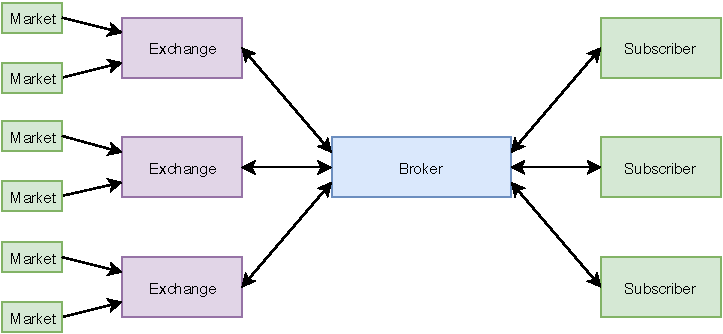
\includegraphics[width=\textwidth]{marketpull.pdf}
    \caption[\project's Publish/Subscribe system]{exchanges illustrate publishers; they extract market data that gets propagated to the broker. The subscribers can express interest in specific markets to the broker. And the broker forwards data from the publishers to the subscribers.}
    \label{fig:ccxt}
\end{figure}

The method we use to extract market data from ccxt's uniform \ac{api} is the ticker function, which contains similar information given by Binance, but we only use the  \ac{ohlc} values. With the reverse map we created, we also estimate the ratio of how many exchanges that lists a specific market as this feature was explicitly described in \autoref{tab:pd_characteristics} as a \ac{pd} characteristics.

\subsubsection{CoinMarketCap}
The final slave retrieves data from \href{https://coinmarketcap.com/}{CoinMarketCap}, which is a popular cryptocurrency tracking site and contains statistics regarding a coin's capitalization, circulation, etc. We must use CoinMarketCap's private \ac{api} as they recently deprecated their public \ac{api}. Using their private \ac{api} requires an \ac{api} key for user identification. With the \ac{api} key, CoinMarketCap are able to track users request rate, which is troublesome as their request limit to a free subscription is low, only $333$ request daily is allowed to issue. They have defined a severe complex request system. Where a user has a load of credits, and the amount of credit one has, depends on the type of subscription one has. A user also has a daily, weekly, and monthly request rate system, which also depends on the type of subscription on have. 

There are some Python modules in existence that allows one to extract data from CoinMarketCap, but they completely ignore the request system, which when used will be problematic as we continuously will exceed the request limit and credit system, which ultimately results in a permanent ban from using their \ac{api}.

Thus, we create a module that supports throttling of requests, which adjusts to both the credit system and the number of requests one can issue. And we cache every request in an SQLite database because CoinMarketCap mostly provides data that rarely or slightly change, and the cache functionality comes with an exceed factor.

These are the four endpoints at CoinMarketCap:
\begin{itemize}
    \item Cryptocurrency
    \item Exchanges
    \item Globals
    \item Tools
\end{itemize}

We use the modules requests, requests\_cache, and ratelimit. The requests module for making requests to CoinMarketCap's \ac{api}. Requests\_cache is a monkey patch to the request module, and caches every request made by it. The ratelimit allows us to define function decorators that restricts the number of function calls within an interval.

This slave fetches data from the endpoints, cryptocurrency and global. In the global endpoint, we use the global-metric function that contains the total market capitalization of all coins. And in the cryptocurrency endpoints, we fetch cryptocurrencies' latest market data that contains fields like capitalization, which says how a coin is worth. CoinMarketCap does provide market data, but since we cache every request and the request limit is limited to $333$ a day, we can not use it as it results in us using stale trading data.

\section{Data Preparing}
After gathering enough data, we start to prepare it for \ac{ml}. Each market has a file containing data from the sources we recently described. And since we prepare the data in the files equally, we can speed up the operations by processing the files in parallel. Each file we have to process can be small in general, but combining them all, they become quite large, and it is infeasible to load them all into memory. Hence, we only process a fixed number of files in parallel.

We parallelize every operation by creating, yet again, a master/slave structure where the master process spawns the same number of child processes (slaves) as there are markets. The slaves are initialized with a market, a semaphore to control the number of processes to run inside a critical section, and a queue to signalize back to the master when it's done. Inside the critical section, the child loads the dataset, execute the desired operation, and stores the result. After the slave leaves the critical section, it signalizes back to the master. The slaves use the module Pandas to load the datasets into a dataframe. With a data frame, a slave can index features by their column name, which makes it convenient when we do cleansing and feature engineering. 

The first operations involve cleansing the data. We cleanse by removing corrupted files. We also remove the features that are not needed, e.g, in \autoref{code:binance_tick}, the constant categorical field \texttt{symbol} are not needed when classifying \ac{pd}. The last cleansing process we do is to interpolate the data. Values involving price and volume gets linearly interpolated as we describe in \autoref{ch:design}.

The second series of operation we do is to create new features. We calculate the \ac{poc} like described in \autoref{ch:design} on all the values we interpolated. Then we create new features from using the timestamp that we added along with the data when it was stored. Finally, we create a new feature that describes the imbalance of the order book.

\section{Collecting pump-and-dumps}
We implement the anomaly detection algorithm to detect anomalous intervals contains \ac{pd}, this algorithm was described in \autoref{ch:design}. The algorithm marks an interval anomalous if there is a significant increase in price and volume in that period compared to the previous periods. We can not use the anomaly detection algorithm with the real-time data that was collected, as this data is not compliant with the algorithm. Instead, we retrieve historical \ac{ohlc} data from Binance that span over the period we gathered data.

This algorithm uses sliding a window containing a fixed number of \ac{ohlcv} values. We created a sliding window module which wraps around a python list. The list has fixed size, and when adding new elements to the list, the last element will be removed, just like a fixed size \ac{fifo} structure.

\autoref{code:binance_kline} illustrates a response from Binance that contains historical \ac{ohlc} values. With these values and a sliding window, we start to continuously add \ac{ohlcv} values that span over the period we collected data. And we iteratively calculate whether the newest added \ac{ohlc} is an anomaly compared to the other \ac{ohlcv} values in the window. The fields that we use from \autoref{code:binance_kline} are \texttt{close} and \texttt{high} to calculate whether the price surpasses a specified threshold, while we use the field \texttt{volume} when calculating whether volume exceeds a specified volume threshold.

\begin{lstlisting}[language=json, caption={Historical kline response from Binance.}, label=code:binance_kline]
[
  [
    1499040000000,      // Open time
    "0.01634790",       // Open
    "0.80000000",       // High
    "0.01575800",       // Low
    "0.01577100",       // Close
    "148976.11427815",  // Volume
    1499644799999,      // Close time
    "2434.19055334",    // Quote asset volume
    308,                // Number of trades
    "1756.87402397",    // Taker base volume
    "28.46694368",      // Taker quote volume
  ]
]
\end{lstlisting}

As we have previously mentioned, anomaly detection algorithms tend to have a high occurrence of false positive compared to true positive. So we remove the false positives anomalies by first plotting finer-grained \acp{ohlc} values over the periods that were flagged anomalous in each market. Then, removing the anomalies that we believe is not a \ac{pd}, while retaining the anomalies that we believe is a \ac{pd}. We plot the \ac{ohlc} values by using the matplotlib module.

After filtering \acp{pd}, we label the features that we have created. We use the same master/slave method, which we used during the feature engineering stage. Where each process is initiated with a semaphore and queue, but also the \ac{pd} anomalies. To label the dataset, slaves loads its assigned dataset and identify the interval where the \ac{pd} occurred, and find the points where the most significant change in price percent happened. From the highest point, we label the points as positive from where the change in percent was positive until it becomes negative.

\section{Deep Learning}
We normalized each market using the min-max method described in \autoref{ch:design}. We have to process the data over two iterations, in the first iteration, we iterate over all the markets to find the largest and smallest value in the features. Then, in the second iteration, we normalize the features.

To create a balanced dataset, we undersample the data. So, we first have to collect all the positive samples from the datasets. Then we select random negative sequences from them until the number of negative and positive samples are approximately equal.

We use the deep learning library Keras for building the model, and the first layer contains \ac{lstm} cells and the output layer contains a single perceptron. Training a \acp{lstm} network requires us to reshape our 2D input data, into a 3D shaped matrix. The 3D shape represents matrices inside a matrix. A sample in a 3D space is a matrix containing a batch of vectors within a time lag. Then the third dimensions is a batch of these new samples. After shaping the data, we can finally train our model.